\section{Durchführung}
\label{sec:Durchführung}
\subsection{Aufbau}
Im Versuch ist ein Spannungsgenerator gegeben, der für die erste Messreihe nur über einen Tiefpass mit einem Oszilloskop verbunden ist, zu sehen in Abbildung \ref{foto1} 
Für die Aufnahme der zweiten Messreihe und zur messung zur Bestätigung der Integratorfunktion wird auch noch eine direkte Verbindung zwischen dem Spannungsgenerator und dem Oszilloskop eingeführt, zu sehen in Abbildung \ref{foto2}.
\begin{figure}
\centering
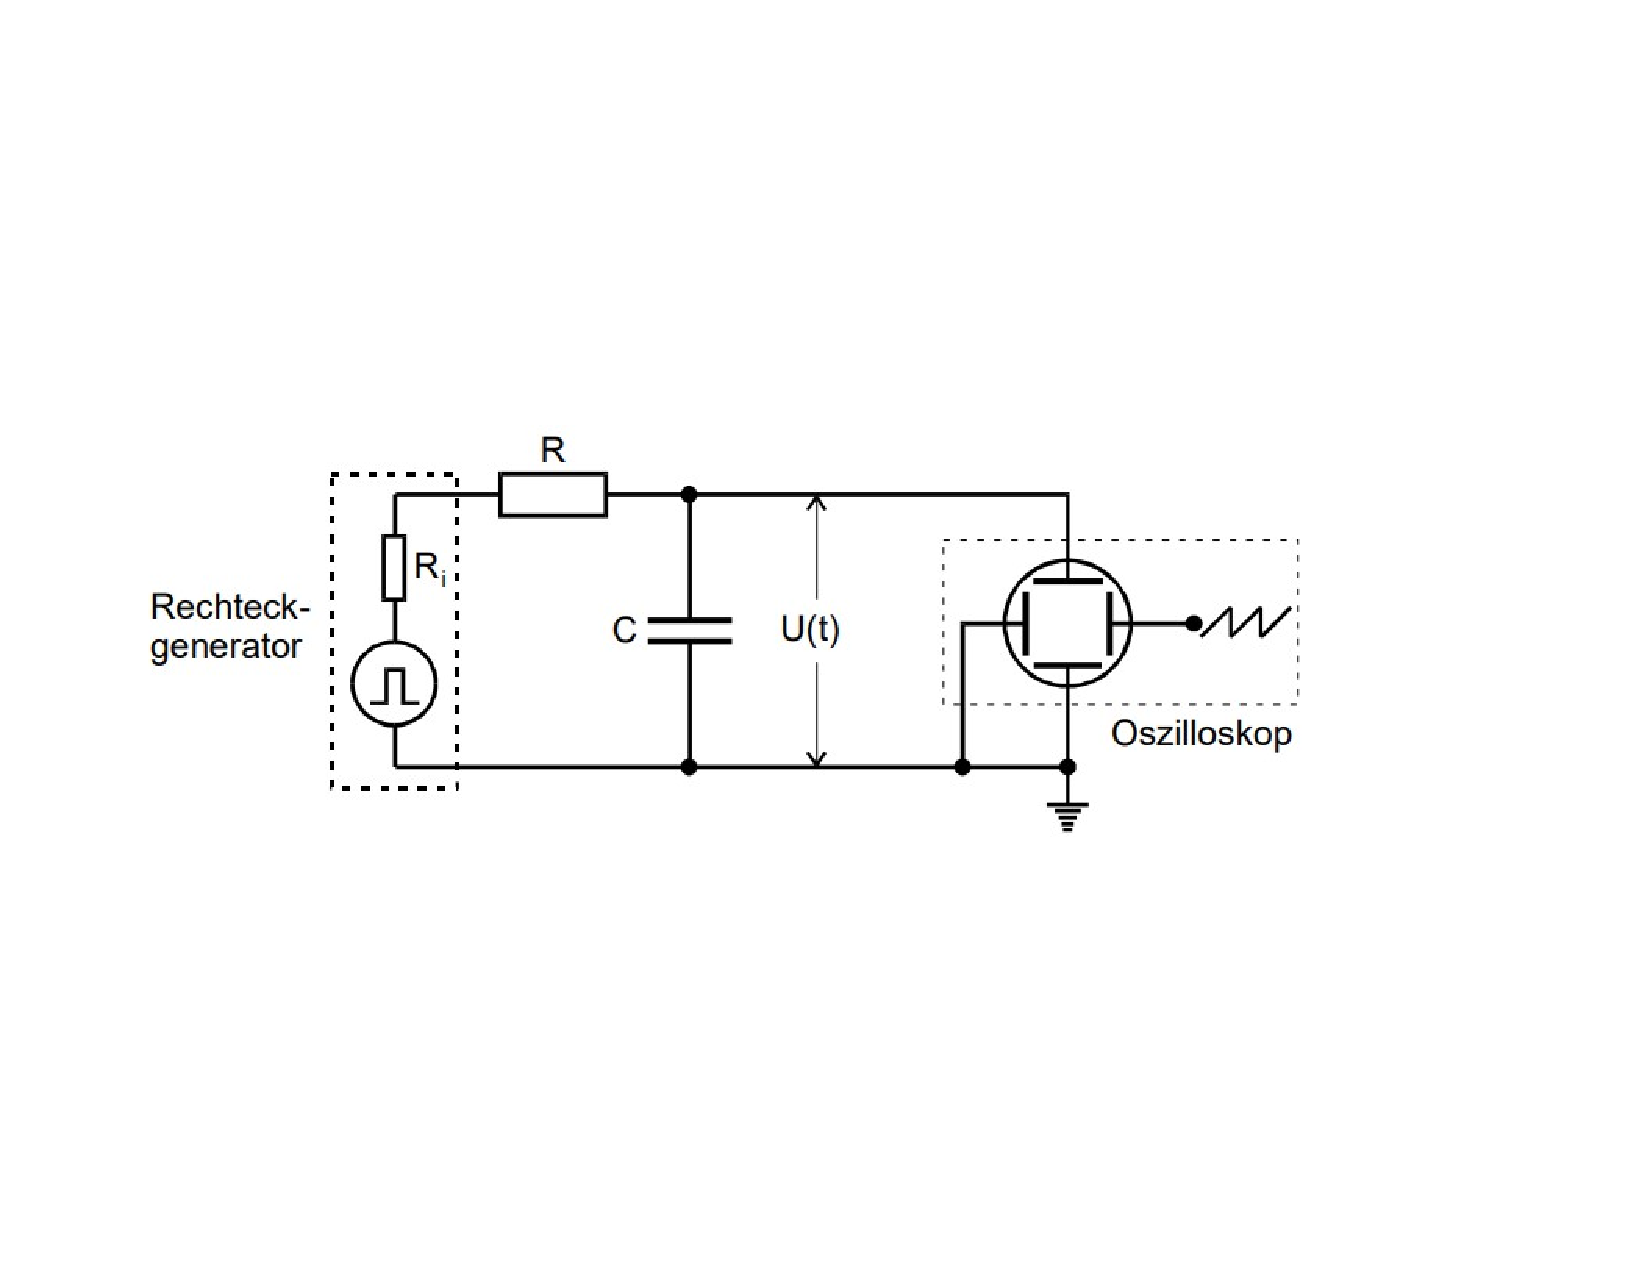
\includegraphics[width = 10cm]{V353foto4.pdf}
\caption{Aufbau für die erste Messreihe \cite{V353}}
\label{foto1}
\end{figure}

\begin{figure}
    \centering
    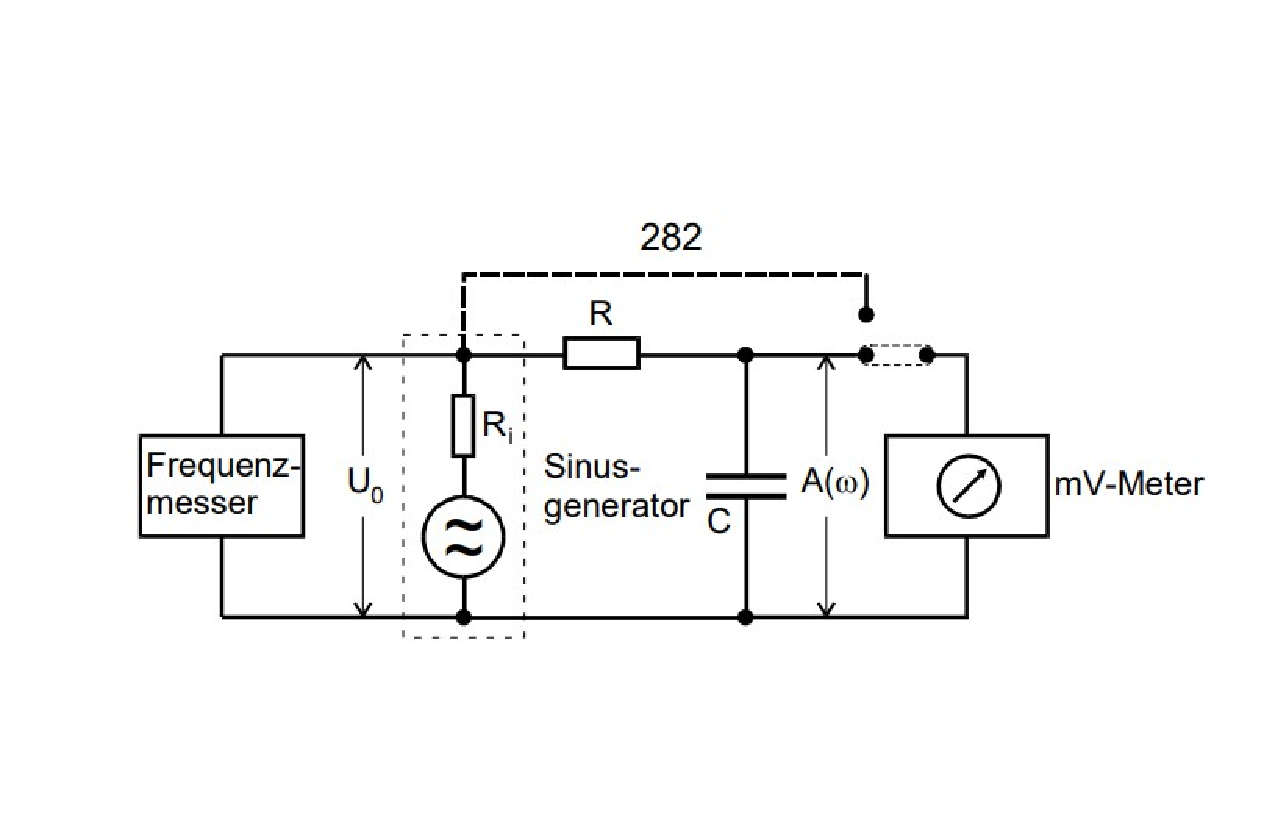
\includegraphics[width = 10cm]{V353foto5.pdf}
    \caption{Aufbau für die zweite Messreihe \cite{V353}}
    \label{foto2}
    \end{figure}

\subsection{Messreihe zur Entladekurve}
In der ersten messreihe werden Wertepaare der Spannung $U_c$ und der Zeit $t$ von der auf dem oszilloskop dargestellten Entladekurve abgelesen. 
Die Frequenz bleibt dabei konstant auf $77.2\unit{\hertz}$.
\subsection{Messreihe der Phasenverschiebung und der Spannungsamplitude}
In der zweiten Messreihe werden die Werte für die Phasenverschiebung zwischen der Generator- und der Kondensatorspannung und die Spannungsamplitude der Kondensatorspannung bei einer variierenden Frequenz $F$ 
von den auf dem oszilloskop dargestellten Kurven abgelesen. Die Messung wurde bei $F = 22000\unit{\hertz}$ aus technischen Gründen vorzeitig abgebrochen.
Gleichzeitig wird die Generatorspannungsamplitude abgelesen um zu versichern dass diese konstant bleibt.
\subsection{Messung zur Verifikation der Integratorfunktion}
Nun werden verschiedene Spannunsformen vom Spannungsgenerator erzeugt, die generierte Spannung wird gemeinsam mit der durch den Tiefpass integrierten Spannung auf dem Oszilloskop angezeigt,
die angezeigten Bilder werden Fotografiert. Es werden die Spannungen für eine Sinus- eine Dreieck- und eine Reckteckspannung fotografiert.

